\newpage
\section{Crop Growth}
Equations related to crop growth modeling. Most equations, unless otherwise noted, are derived from \cite{GENECROP}.
\subsection{Background}
These equations are based off the RI-RUE model developed by Monteith.
\begin{gather}
    RG_t = RUE_t \times RAD_t \times (1-\exp{[-k\times LAI_t]}) \\
    DBM = \int_0^t RG_t \times dt
\end{gather}
where
\begin{conditions*}
RG & Rate of plant growth (g) \\
RUE & Radiation use efficiency (g/MJ) \\
RAD & Radiation (MJ) \\
k & Radiation extinction constant
    \footnote{As explained in \cite{penning_de_vries}, radiation will be intercepted at different rates depending on the
    structure (size and shape) of the leaf canopy. For erect, horizontal leaves, this value ranges from 0.6 to 0.8.} \\
LAI & Leaf area index (m$^2$/m$^2$) \\
DBM & Dry biomass (g)
\end{conditions*}
Leaf area index is calculated as a function of the specific leaf area ($SLA$), which is itself a function of the development stage of the crop ($DVS$), and the leaf biomass at time t ($LeafB_t$).
\begin{equation}
    LAI_t = SLA_t \times LeafB_t
\end{equation}
where
\begin{conditions*}
SLA & Specific leaf area (m$^2$/g) \\
LeafB & Leaf biomass per unit area (g/m$^2$)
\end{conditions*}
\subsection{Assumptions}
\begin{itemize}
    \item Many constants and parameters are assumed based off a specific crop in specific conditions (see "Interpolated Values")
    \item Crop parameters are constant throughout all crop cycles
\end{itemize}
\subsection{Procedure}
To begin, the development stage ($DVS$) is calculated using the following relationship (Fig. \ref{fig:DVS}):
\begin{figure}[h]
    \centering
    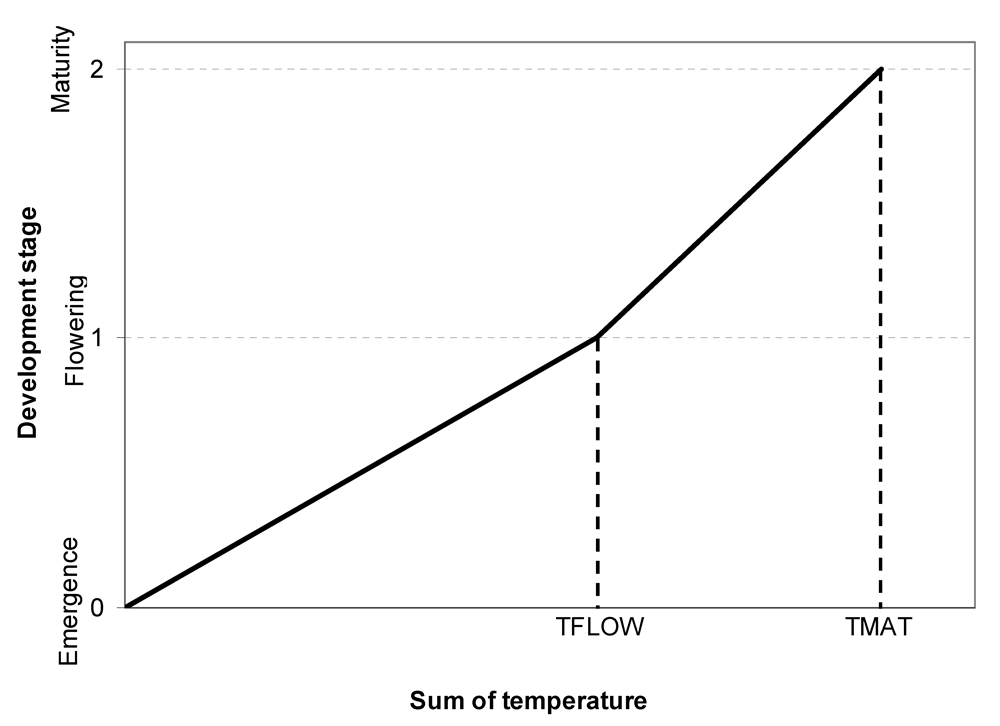
\includegraphics[width=\textwidth]{DVS.jpg}
    \caption{Plot of $GDD$ (i.e. Sum of temperature) vs. $DVS$ \cite{GENECROP}}
    \label{fig:DVS}
\end{figure}
\begin{equation}
    DVS_t = \left.
    \begin{cases}
        GDD_t / GDD_{flow}, & \text{if } GDD_t < GDD_{flow} \\
        1 + (GDD_t - GDD_{flow})/(GDD_{mat} - GDD_{flow}), & \text{if } GDD_t \geq GDD_{flow}
    \end{cases}
    \right\}
\end{equation}
where
\begin{conditions*}
    GDD_t & Growing degree days at time t (\degree C-day) \\
    GDD_{flow} & Growing degree days at flowering (\degree C-day) \\
    GDD_{mat} & Growing degree days at maturity (\degree C-day)
\end{conditions*}
The flowering and maturity GDDs are unique to each crop and have been acquired for wheat, soy, and corn from various sources. To calculate the growing degree days for a crop ($GDD$), the following equation is used.
\begin{equation}
    GDD_t = \int_0^t [\min{(T_{air},T_{max})} - T_{base}]\, dt
\end{equation}
where
\begin{conditions*}
    T_{air} & Mean air temperature (\degree C) \\
    T_{max} & Cutoff temperature beyond which crop does not benefit (\degree C) \\
    T_{base} & Cutoff temperature below which crop does not benefit (\degree C)
\end{conditions*}
Values for $T_{max}$ and $T_{base}$ are available in various sources for wheat, corn, and soy, and for the purposes of this simulation, the trapezoid method was used to estimate the above integral.

A step-wise process is then taken involving the partitioning of total available photosynthetic energy ($POOL$) into the leaves ($LeafB$), stems ($StemB$), roots ($RootB$), and storage organs ($StorB$). 
\begin{equation}
\label{eq:POOL}
    POOL_{t+\Delta t}=POOL_t + (RG_t \times \Delta t)
\end{equation}
\begin{gather}
\label{eq:LeafB}
    LeafB_{t+\Delta t}=LeafB_t + (PartL_t \times \Delta t) \\
\label{eq:StemB}
    StemB_{t+\Delta t}=StemB_t + (PartS_t \times \Delta t) \\
    RootB_{t+\Delta t}=RootB_t + (PartR_t \times \Delta t) \\
\label{eq:StorB}
    StorB_{t+\Delta t}=StorB_t + (PartSO_t \times \Delta t)
\end{gather}
where $PartL$, $PartS$, $PartR$, and $PartSO$ are the daily flows of biomass to the leaves, stems, roots, and storage organs, respectively. To calculate these:
\begin{gather}
    PartL_t= POOL_t \times CPL_t \times (1-CPR_t) \\
    PartS_t= POOL_t \times CPS_t \times (1-CPR_t) \\
    PartR_t= POOL_t \times CPR_t \\
    PartSO_t= POOL_t \times CPSO_t \times (1-CPR_t)
\end{gather} 
where $CPL$, $CPS$, $CPR$, and $CPSO$ are the partitioning coefficients for the leaves, stems, roots, and storage organs, which depend on the development stage ($DVS$). Values for these are fixed and interpolated for values of $DVS$ (see "Interpolated Values").

After calculating these values, (\ref{eq:POOL}) can be transformed to incorporate partitioning of available resources.
\begin{equation}
    POOL_{t+\Delta t}=POOL_t + (RG_t - PartL_t - PartS_t - PartR_t - PartSO_t) \times \Delta t
\end{equation}
\subsubsection{Leaf Senescence}
Incorporating the relative rate of leaf biomass decline due to aging ($rrsenl$), the rate of leaf biomass growth (\ref{eq:LeafB}) can be transformed:
\begin{gather}
    LeafB_{t+\Delta t} = LeafB_t + (PartL_t - RSenL_t) \times \Delta t \\ 
    RSenL_t = rrsenl_t \times LeafB_t
\end{gather}
\subsubsection{Accumulation and redistribution of reserves}
In later stages of development, biomass can translocate between the stem or roots and storage organs. Thus, incorporating this factor ($RTransloc$), (\ref{eq:StemB}) and (\ref{eq:StorB}) become:
\begin{gather}
    StemB_{t+\Delta t} = StemB_t + (PartS_t - RTransloc_t) \times \Delta t \\
    StorB_{t+\Delta t} = StorB_t + (PartSO_t - RTransolc_t) \times \Delta t \\
    RTransloc_t = \left.
    \begin{cases}
        0 & DVS \leq 1 \\
        0.005 \times MaxStemB & DVS > 1
    \end{cases}
    \right\} \\
    MaxStemB_{t+\Delta t} = MaxStemB_t + PartLS \\
    PartLS = PartL + PartS
\end{gather}

\subsection{Evapotranspiration}
Evapotranspiration ($ET_0$) is calculated using the Penman-Monteith equation, following the procedure of \cite{penman_monteith}. The so-called FAO 56 Penman-Monteith equation is a standardized method of calculating reference evapotranspiration for "a hypothetical reference crop with crop height of 0.12 m, a fixed surface resistance of 70 s m$^{-1}$ and an albedo value[...] of 0.23." It takes the form below\footnote{For a daily time step, the numerator constant 37.5 is multiplied by 24}:
\begin{equation}
    ET_0=\frac{0.408(R_n-G)+\gamma \frac{37.5}{T+273}u_2 (e_s - e_a)}{\Delta + \gamma (1+0.34 u_2)}
\end{equation}
where
\begin{conditions*}
    ET_0 & Reference evapotranspiration (mm hr$^{-1}$) \\
    R_n & Net radiation at the crop surface (MJ m$^{-2}$ hr$^{=1}$) \\
    G & Soil heat flux density (MJ m$^{-2}$ hr$^{=1}$) \\
    T & Mean hourly air temperature at 2 m height (\degree C) \\
    u_2 & Wind speed at 2 m height (m s$^{-1}$) \\
    e_s & Saturation vapor pressure (kPa) \\
    e_a & Actual vapor pressure (kPa) \\
    \Delta & Slope of saturation vapor pressure curve (kPa \degree C$^{-1}$)\\
    \gamma & Psychometric constant (kPa \degree C$^{-1}$)
\end{conditions*}

Crop-specific ET is then computed using the equation
\begin{equation}
    ET_c = K_c \times ET_0
\end{equation}
where $K_c$ is the crop coefficient. Values for $K_c$ can be approximated using the regression equations of \cite{nmsu}. The equations for wheat, soy, and corn are shown below.
\begin{multline}
    \textbf{Wheat:} \; K_c = 2.7\times 10^{-1} - 4.8\times 10^{-4}GDD_t + \\ 6.27 \times 10^{-7}GDD_t^2 - 1.3 \times 10^{-10} GDD_t^3
\end{multline}
\begin{multline}
    \textbf{Corn:} \; K_c = 1.2\times 10^{-1} + 1.68\times 10^{-3}GDD_t - \\ 2.46 \times 10^{-7}GDD_t^2 - 4.37 \times 10^{-10} GDD_t^3
\end{multline}
\begin{multline}
    \textbf{Soy:} \; K_c = 4.35\times 10^{-2} + 1.37\times 10^{-3}GDD_t - \\ 5.3 \times 10^{-7}GDD_t^2 - 5.43 \times 10^{-11} GDD_t^3
\end{multline}

\newpage
\subsection{Interpolated Values}
The following values are used in the crop growth equations. They are based on a model for rice production in South Asia \cite{RICEPEST, GENECROP}.
\begin{center}
\begin{tabular}{llllll}
\textbf{DVS} & \textbf{CPR} & \textbf{CPPL} & \textbf{CPPP}  & \textbf{rrsenl} & \textbf{SLA} \\ \hline
0            & 0.3          & 0.55          & 0                           & 0   & 0.037           \\
0.05         &              &               & 0                             &                \\
0.1          & 0.263        & 0.536         & 0                            & 0              \\
0.15         &              &               & 0                         &                \\
0.2          & 0.225        & 0.521         & 0                          & 0              \\
0.25         &              &               & 0                           &                \\
0.3          & 0.188        & 0.507         & 0                       & 0              \\
0.35         &              &               & 0                             &                \\
0.4          & 0.15         & 0.493         & 0                          & 0              \\
0.45         &              &               & 0                         &                \\
0.5          & 0.112        & 0.479         & 0                  & 0              \\
0.55         &              &               & 0                        &                \\
0.6          & 0.075        & 0.464         & 0                     & 0              \\
0.65         &              &               & 0                            &                \\
0.7          & 0.038        & 0.45          & 0                       & 0              \\
0.75         &              &               & 0                            &                \\
0.8          & 0            & 0.3           & 0.143                   & 0              \\
0.85         &              &               & 0.286                        &                \\
0.9          & 0            & 0.15          & 0.429                   & 0              \\
0.95         &              &               & 0.571                      &                \\
1            & 0            & 0             & 0.714                     & 0         & 0.018     \\
1.05         &              &               & 0.857                      &                \\
1.1          & 0            & 0             & 1                         & 0.013          \\
1.15         &              &               & 1                         &                \\
1.2          & 0            & 0             & 1                         & 0.026          \\
1.25         &              &               & 1                            &                \\
1.3          & 0            & 0             & 1                         & 0.04           \\
1.35         &              &               & 1                           &                \\
1.4          & 0            & 0             & 1                          & 0.04           \\
1.45         &              &               & 1                            &                \\
1.5          & 0            & 0             & 1                          & 0.04           \\
1.55         &              &               & 1                           &                \\
1.6          & 0            & 0             & 1                          & 0.04           \\
1.65         &              &               & 1                            &                \\
1.7          & 0            & 0             & 1                         & 0.04           \\
1.75         &              &               & 1                          &                \\
1.8          & 0            & 0             & 1                           & 0.04           \\
1.85         &              &               & 1                         &                \\
1.9          & 0            & 0             & 1                           & 0.04           \\
1.95         &              &               & 1                            &                \\
2            & 0            & 0             & 1                          & 0.04      & 0.017    
\end{tabular}
\end{center}